\documentclass[11pt]{article}

\usepackage[margin=0.75in]{geometry}
\usepackage{graphicx}
\graphicspath{ {images/} }

\title{The title of your project proposal}
\author{
  Jara, Jon\\
  \texttt{jonmigueljara}
  \and
  Shishido, Juan\\
  \texttt{juanshishido}
  \and
  Xu, Wendy\\
  \texttt{berithsu}
}

\bibliographystyle{siam}

\begin{document}
\maketitle

\abstract{
The goal of this research is to analyze brain activities associated with
decision-making. In particular, we draw upon the experiment of mixed gambles to
investigate the relationship between neural and behavioral loss aversion. The
relationships are observed by neural activities, measured as fMRI data, when
subjects are exposed to gambles. Our project attempts to apply linear
regression and multi-voxel pattern analyses to study loss-and-gain sensitivity
levels inside the brain.
}

\section{Introduction}

Our research idea is based on the 2007 paper The Neural Basis of
Loss Aversion in Decision-Making Under Risk, written by Sabrina M. Tom, Craig
R. Fox, Christopher Trepel, and Russell A. Poldrack\cite{tom}. Our goal is to
reproduce the major part of the paper with possible simplifications and also
develop some original analysis on the same data.

A significant portion of the paper is devoted to analyzing neural
indicators of loss aversion and correlating that neural loss aversion to
behavioral loss aversion. Test subjects are presented with gambles with equal
chances of winning and losing and different amounts of money to gain and lose.
These gamble offers and the subject’s decision of whether or not to accept the
gamble are recorded, as well as the subject’s neural activities during the
tasks. Behavioral risk aversion is measured through modeling the participant’s
decision on the amount of proposed gain and loss of the gambles. On the other
hand, neural risk aversion is measured through modeling the participant’s fMRI
data on the amount of proposed gain and loss of the gambles. The researchers
find that behavioral loss aversion is statistically correlated with neural risk
aversion. Another finding is that that some areas of the brain are particularly
sensitive to both gains and losses, exhibiting increasing activity as potential
gains increase and decreasing activity as potential losses increase. Neural
activities in these areas can reasonably be used to predict behavioral loss
aversion.

The main approach used by the researchers is called the ``matrix analysis.''
The gain/loss matrix, from where gambles are randomly drawn and displayed to
the experiment subject, is collapsed from a 16 x 16 into a 4 x 4 matrix and
trials for all subjects and runs are grouped according to this smaller matrix,
resulting in 16 separate conditions. Separate estimation of the evoked response
for each of these conditions enables the comparison between ``good'' versus
``bad'' gambles. Another separate approach is the ``parametric analysis,''
where all the trials are modeled by orthogonal parametric regressors
representing the size the potential gain, the size of the potential loss, and
the Euclidean distance of the gain and loss combination from the diagonal of
the gain/loss matrix. Both methods are carried out by time-series analysis
using FILM (FMRIB’s Imporoved Linear Model).

We will reproduce this part of the paper using mostly linear regression and
logistic models and evaluate our results against the paper’s results as well as
using error analysis. We will also visualize our research results consistently
with 2-D and possibly 3-D graphs. We would also like to experiment with
multi-voxel pattern analysis on the fMRI data, which helps detect patterns of
brain activity by jointly analyzing multiple voxels at the same time. 

\section{Data}

\subsection{Description}

The data set includes 3 sample runs for each subject, with 16 subjects in
total. The subjects consist of 9 females and 7 males. For each run, the subject
is presented with a series of gambles with different combinations of gains and
losses, each combination randomly drawn from a gain/loss matrix of size 16 x
16. For the purpose of analysis, the data are collapsed into a 4 x 4 matrix.
The subject’s fMRI data generated during the tasks is available for each run.

The typical brain image consists of 64 x 64 voxels for each brain slice and 34
slices in total. Repetition time (TR) is 2 seconds. Two volumes are discarded
at the beginning of each run.

\subsection{Acquiring}

A primary goal of ours is to ensure that individuals who wish to replicate or
improve upon our work can easily do so. To that end, in terms of data access,
we have created a bash script that fetches the data from www.openfmri.org and
untars it. It runs only if the data directory doesn't already exist. The script
also downloads the checksums and we've written a Python script to check that
the hashes match. We will incorporate the Python script in the Makefile for
downloading the data.

\section{Methods}

\subsection{Preprocessing}

We are considering several preprocessing techniques to use on our data.

\subsubsection{Smoothing}

After initial plots, we observed that the data was noisy. Smoothing in space
reduces the noise by averaging data---in this case, voxels---with its
neighbors, while preserving signal. This is typically done using a Gaussian
function. The selected width of the distribution determines how much the data
are smoothed.

There are several benefits related to smoothing. Below, we list the ones that
are relevant for our analysis.

\begin{itemize}
  \item increased sensitivity
  \item making the error distribution normal
\end{itemize}

We are also aware of the following disadvantages.

\begin{itemize}
  \item{reduced spatial resolution}
  \item{edge artifacts}
\end{itemize}

Typically, for single-subject analyses, a width of 4 mm is used. This
information came from the Brain Voyager website\cite{bvsmoothing}.

The first step we took in pre-processing the blood-oxygen-level dependent
(BOLD) image data was to smooth the BOLD data using a Gaussian filter by two
standard deviations in all three spatial dimensions. Figure
~\ref{fig:smoothing-before} and Figure ~\ref{fig:smoothing-after} show how
smoothing vastly improves the interpretability of the single brain images (note
that these images were not the final plots used in analysis, these are just to
show how images looked before and after smoothing).

\begin{figure}[h]
\caption{Before Smoothing}
\centering
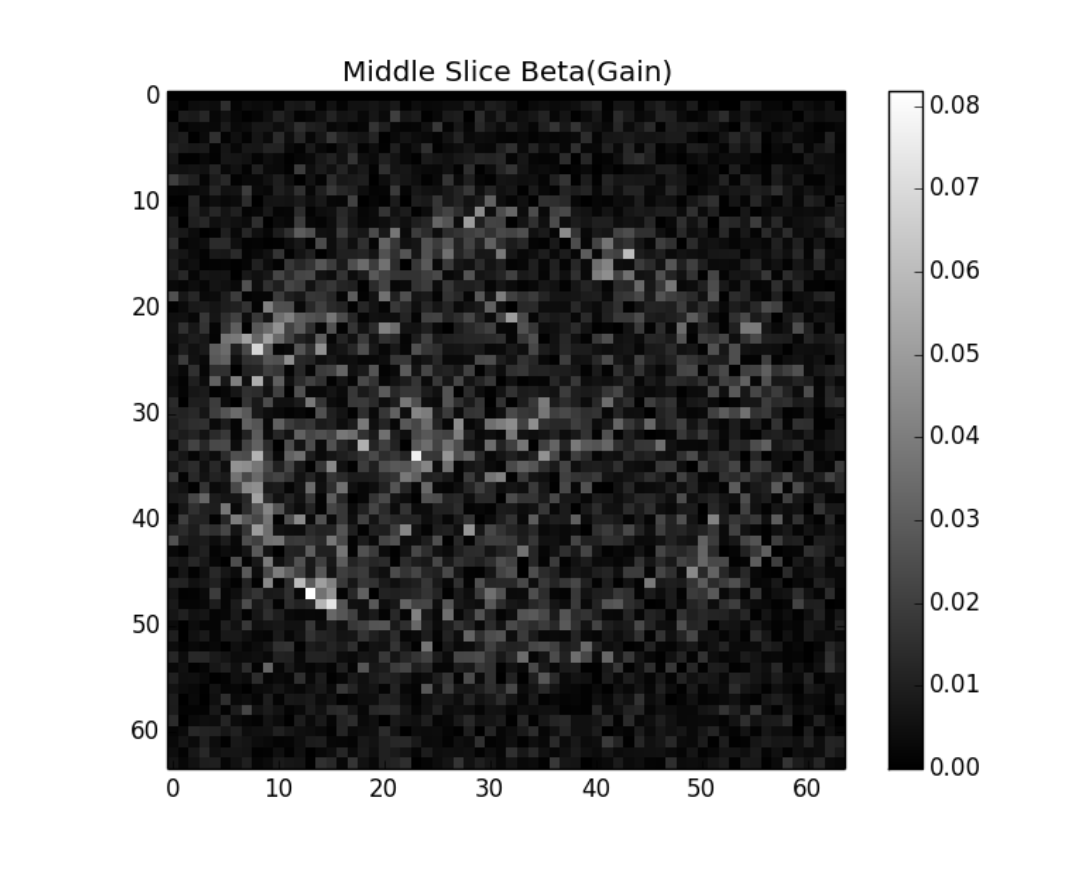
\includegraphics[width=0.5\textwidth]{smoothing-before.png}
\label{fig:smoothing-before}
\end{figure}

\begin{figure}[h]
\caption{After Smoothing}
\centering
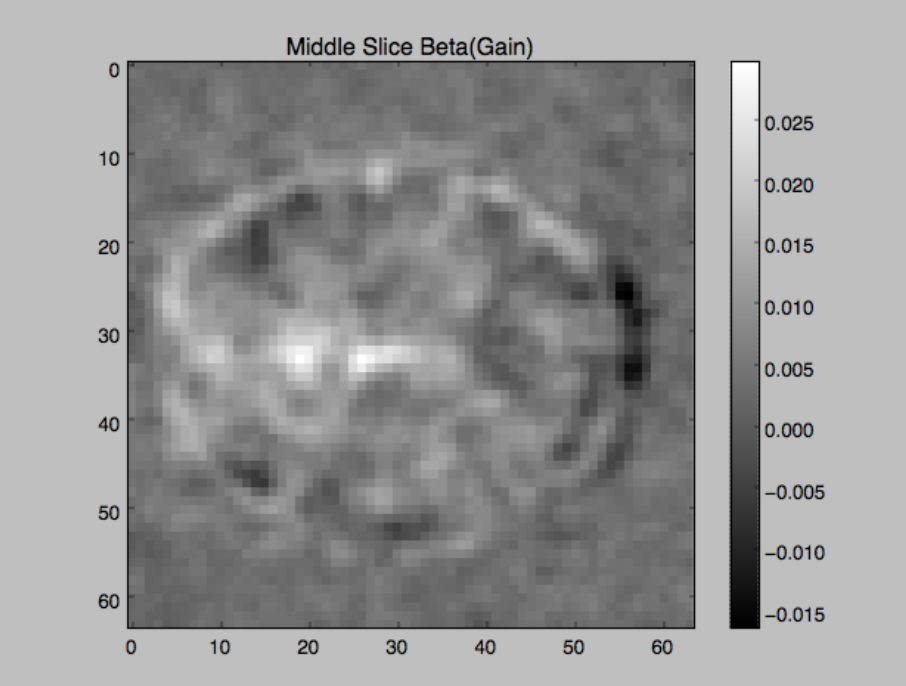
\includegraphics[width=0.5\textwidth]{smoothing-after.png}
\label{fig:smoothing-after}
\end{figure}

\subsubsection{Principle Component Analysis}

We are also considering using principle component analysis (PCA) to reduce the
dimensionality of our data. We will investigate the standard PCA approach,
e.g., the one found in Scikit-Learn's decomposition submodule. Research by
Viviani, Gron, and Spitzer\cite{viviani}, however, has shown that
\textit{functional} principle component analysis is more effective than the
standard approach. We plan to experiment with this approach.

\subsubsection{Motion Correction}

Another way in which we will attempt to increase the signal from our data is to
correct for motion. Nipy includes the function \texttt{FmriRealign4d} that
corrects for both motion and slice timing.

\subsection{Analysis}

In their primary analysis, the researchers build statistical models separately
for each imaging run and create regressors by convolving a delta function
representing trial onset times with a canonical hemodynamic response function.
Similarly, in our research, we will model each run independently and convolve
predictors of interest with a gamma hemodynamic response. We will build linear
regression models for each run using these convolved regressors and
specifically look at the coefficients of those representing gains and losses.
Then we will visualize the coefficients for different slices of the brain to
discover patterns. We also plan on exploring multi-pattern voxel analysis. Both
of these are described in greater detail, below.

\subsubsection{Primary}

The first task is to reproduce the results of the paper using our own tools.
The goal is to find areas of the brain in which neural loss aversion is
correlated to behavioral loss aversion. The result would lead to which parts of
the brain are responsible for making risky decision. The first step is to fit a
logistic regression on the behavioral data using a simple linear regression. We
used a combination of pandas and statsmodels packages to fit a logistic
regression model on the first subject and all the runs combined. Python modules
were used rather than R packages in order to keep the whole project in the same
language and for reproducibility. The logistic regression was modeled in this
manner:

\[ logit(p) = \beta_0 + \beta_1 X_{gain} + \beta_2 X_{loss} + \epsilon \] 

With gain and loss values beings the 2 regressors in the regression. Subject 1
had a gain to loss ratio of 2.33, which was inline with gain to loss ratio
cited by other sources in the paper (around 2.0). The paper was not specific in
how they dealt with multiple runs per subject but we decided that it would be
statistically sound to combine the runs for all the patients. In addition, the
paper conducted pre-processing steps like smoothing and motion correction that
we still need to employ. 

The logistic regression provided results inline with the paper (and past
``risk-averse'') studies and were in the end statistically significant,
however, the main goal of neurological study is to observe how these results
compare with neural signals and brain activity. This part of the analysis has
proven to be less trivial than a simple logistic regression. The challenges
stem mostly from working fMRI data in conjunction with the behavioral variables
``gain'' and ``loss''. We have tried using simple linear regression at each
voxel after convolving the fMRI data, but the results yielded blurry images of
brain slices the general locations of brain activity. While these locations
give a general idea of which parts of the brain are activated during runs of
the experiment, the resulting regressions leaves us with hundreds of beta
coefficients that represent activity without specifying whether the activity is
due to negative loss response and positive gain response. Further research is
needed to perform a similar conjunction analysis that was performed in the
paper. If the complexity of separating the different types of signals is beyond
the scope of our group, we will move on and use the simple regression model
with only one parameter. There is worry that without conjunction analysis we
will not see significant results like those found in the paper and it will be
hard to compare risk aversions to specific loss/gain values if we can
differentiate between the responses. Also, the paper specified specific regions
of the brain with large magnitudes of gain and loss response. To simplify our
analysis, we could restrict our study to whole brain analysis and see if we
find any significant correlation, otherwise we will attempt to segment the same
sections as the ones used in the original study. 

After modeling the fMRI data and hopefully getting valuable coefficients for
loss and gain responses, we will then have to use robust regression to model
the values of these neural response coefficients and the behavioral
coefficients. Robust regression was used in the paper as a way to decrease the
likelihood of any outliers. We might try to simplify this method by using
methods learned in class to remove outlier ourselves and then running a simple
linear regression. In the end, we believe we can reproduce the results of the
paper but we might need to simplify some of the methods, particularly in the
process of quantifying neural risk aversion and segmenting risk-averse areas of
the brain.

\subsubsection{Secondary}

As part of our secondary analysis, we are investigating whether it is possible
to use Multi-Voxel Pattern Analysis (MVPA) on our data. Norman, Polyn, Detre,
and Haxby note that MVPA allows researchers to analyze \textit{vectors} of
voxel activity values instead of individual ones\cite{norman}. There is greater
sentivity with this focus on distributed patterns of activity, making it easier
to detect differences between conditions\cite{bvmvpa}. Typically, linear
classifiers, such as Gaussian Naive Bayes or linear support vector machines,
are used in MVPA analyses\cite{norman}. The features correspond to the brain
activity and the labels to the cognitive state. MVPA also provides the ability
to correlate subject-level classifier estimates across multiple
trials\cite{norman}.

MVPA uses groups of voxels to classify experimental conditions. In our case,
these conditions are gain and loss gambles (or responses to those gambles).
Groups of voxels are typically defined as ``spheres'' from some ``center''
index. The set the default sphere radius to 1. However, it can be of any
arbitrary size, so long as the \textit{diameter} is not larger than the
smallest dimension of the image.

As an example, a sphere with radius 1 will be made up of 27 voxels---9
for each of the three vertical (\(z\)) slices. From the center voxel, the
sphere is made up of the eight surrounding voxels on its plane as well as the
9 corresponding voxels above and below it. While we call the group of voxels a
``sphere,'' we are actually working with cubes.

Because we may not know, a priori, what regions of interest (ROI) in the brain
contain the signals we're interested in, we use a process called
``searchlight'' that fits a classifier on (almost) every sphere across the
entire brain, one at a time. We exclude spheres with center values equal to
zero.

For each subject and each run, the data include 240 time slices. We don't use
all of these for classification. Rather, we restrict the samples (rows) to
those where the time course is equal to one. In other words, the slices where a
gamble occurred.

``Cross-validation'' is a model validation practice to help determine how well
a model will generalize to new, unseen data. It can help avoid the problem of
``overfitting,'' which is the scenario where the model is only good at
predicting the data is was trained (or fit) on. In other words, cases where a
model is not generalizable. During this process, only part of the data is used
to train the model, which is then used to predict the other part. This split is
done randomly. In addition, because we have the access to the ground truth
values, we are able to determine a prediction accuracy. For MVPA, the
cross-validation approach is called ``leave block out.'' This uses groups of
runs to classify other runs.

Once we have our classification accuracy scores, we assign those to the sphere
centers. While prediction accuracy does not necessarily tell us about
activation, ``If this performance of the classifier is significantly above
chance, one concludes that the [blood-oxygen-level dependent] BOLD responses
contain information about the classified states, and infers that the brain area
where the signals originated is somehow involved in the neural representation
of these states''\cite{schreiber2013statistical}.

\subsection{Tools}

We have identified several Python packages we will use for our analysis.

\begin{itemize}
  \item{NumPy}
  \item{pandas}
  \item{Nibabel}
  \item{Statsmodels}
  \item{Scikit-Learn}
  \item{Matplotlib}
  \item{Seaborn}
\end{itemize}

\section{Results}

Thus far, we have run some initial analyses on our data. We have performed
convolution as well as a linear regression. The following is a plot of a middle
slice of the $\hat{\beta}_1$ of a subject's brain.

\includegraphics[width=\textwidth]{beta1_middle_slice.png}

We also have code for our first pass at the logistic regression using the
behavioral data.

\section{Discussion}

\subsection{Challenges}

Many of our issues so far have stemmed from the open ended nature of the
assignment, resulting in less direction than we are used to. This, combined
with the new git workflow, has given us some problems that we are working on
overcoming with a more rigid implementation plan that gives everyone a role.
We are currently using the workflow as best we can, but will be adding many
more Git issues in the coming days in order to better assign work and
facilitate multiple pull requests without merge conflicts. We're having good
success with Python code when we have a good implementation plan. However, a
good deal of our codebase deals with fMRI analysis that we haven't had much
experience working with. This has led to difficulty writing effective tests,
tests that can inspire full confidence in our implementations. We're working on
keeping them simple, using basic modular functions on small datasets to ensure
adequate coverage.

\subsubsection{Team}

We have been working well as a team, and most of our problems are simply
efficiency related. Each of us has applicable skills, we're just trying to get
them all streamlined. This is coming together through the workflow, mainly in
GitHub issues. This allows each of us to work on a different part of the
project at the same time. We have had trouble getting everyone together at the
same time due to erratic schedules, but have been overcoming this using the
workflow.

\subsection{Class Concepts}

We think that we could have used practice in more advanced fMRI analysis
techniques. We've been having some problems with preprocessing, which involves
much more detailed work than we thought. We're looking into some extra Python
libraries to help sort out some advanced preprocessing techniques, smoothing
out confounding variables like respiration and heartbeat. The workflow has been
the most helpful focus, but we think we could have used even more practice.
Because the workflow facilitates efficient team work, we would have liked to
have seen some more group exercises or homework aimed at perfecting the
process.

\bibliography{report}

\end{document}
